% !TeX root = ../../main.tex

\begin{figure}[htb]
\centering 

\begin{subfigure}[b]{0.4\textwidth}
    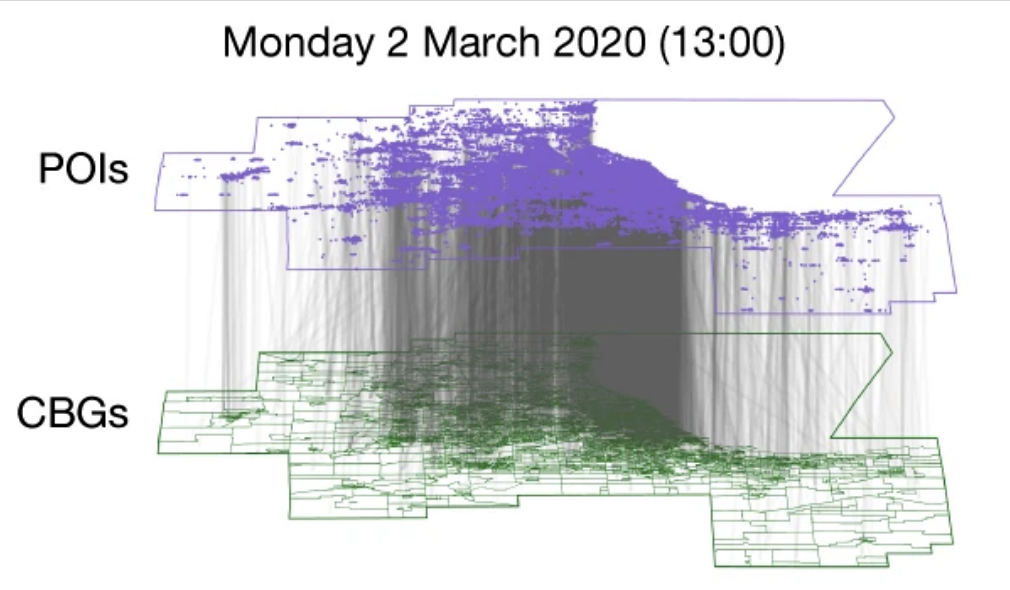
\includegraphics[width=\textwidth]{fig/chang_model/mobility-map.png}
     \caption{Mobility Network}
     \label{fig:chmod-mobility}
\end{subfigure} 
\begin{subfigure}[b]{0.3\textwidth}
    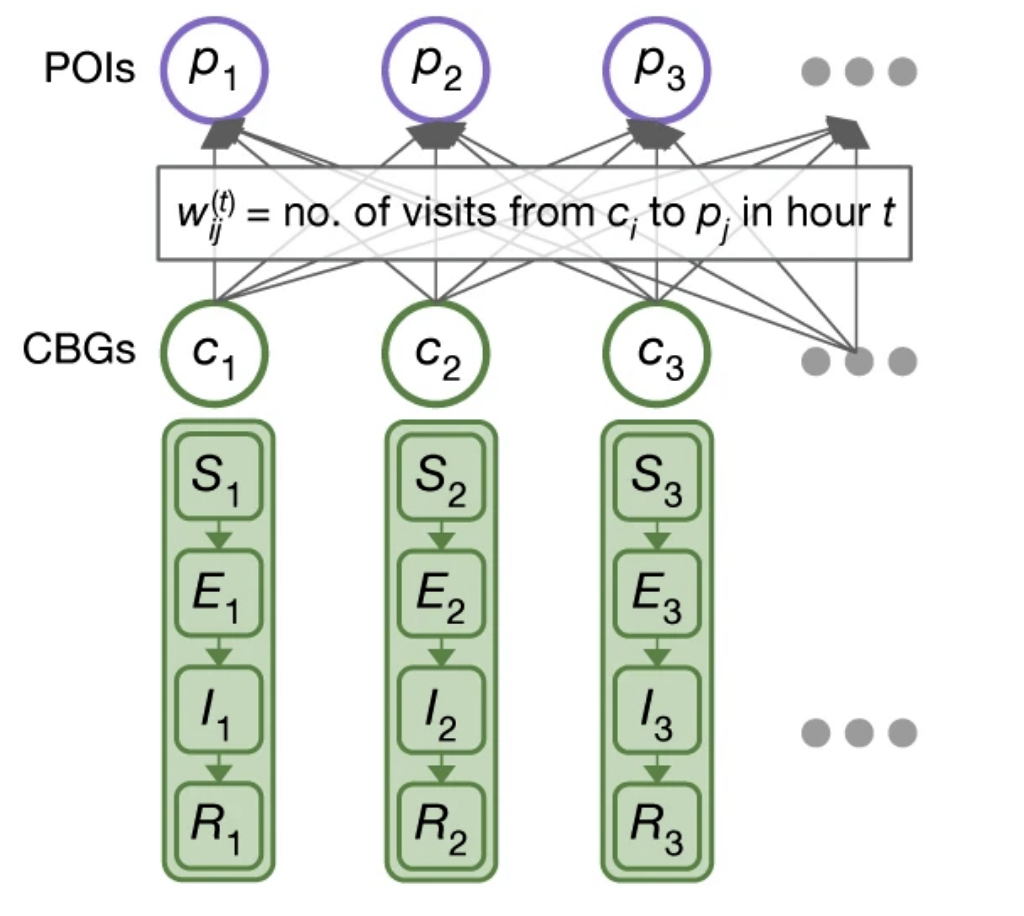
\includegraphics[width=\textwidth]{fig/chang_model/poi-cbg.png}
    \caption{Compartment SEIR model}
    \label{fig:chmod-seir}
\end{subfigure}

\caption{\citeauthor{mobility2020} 的 compartment SEIR 模型. (a) 人口移動的數據, 由 ~\href{https://www.safegraph.com/}{SafeGraph} 的 database 取得 (b) 人口移動會造成居住區域間每個疾病狀態人數的變動。(這個圖片節錄自 Fig. 1a/1b \cite{mobility2020}) }

\label{fig:chmod}

\end{figure}